\documentclass[12pt]{article}
\usepackage[margin=1in]{geometry}
\usepackage{fourier}
\usepackage{graphicx}
\usepackage[import]{xypic}
\usepackage[colorlinks=true, linkcolor=blue, citecolor=blue, urlcolor=blue]{hyperref}

\newenvironment{xyoverpic}[3]
{%
\begin{xy}
\xyimport#1{\includegraphics[#2]{#3}}
}{\end{xy}}

\newenvironment{cxyoverpic}[3]
{%
\begin{center}
\centering\leavevmode\large
\begin{xyoverpic}{#1}{#2}{#3}
}{\end{xyoverpic}
\end{center}}

\begin{document}
\section{Conventions for crossings}

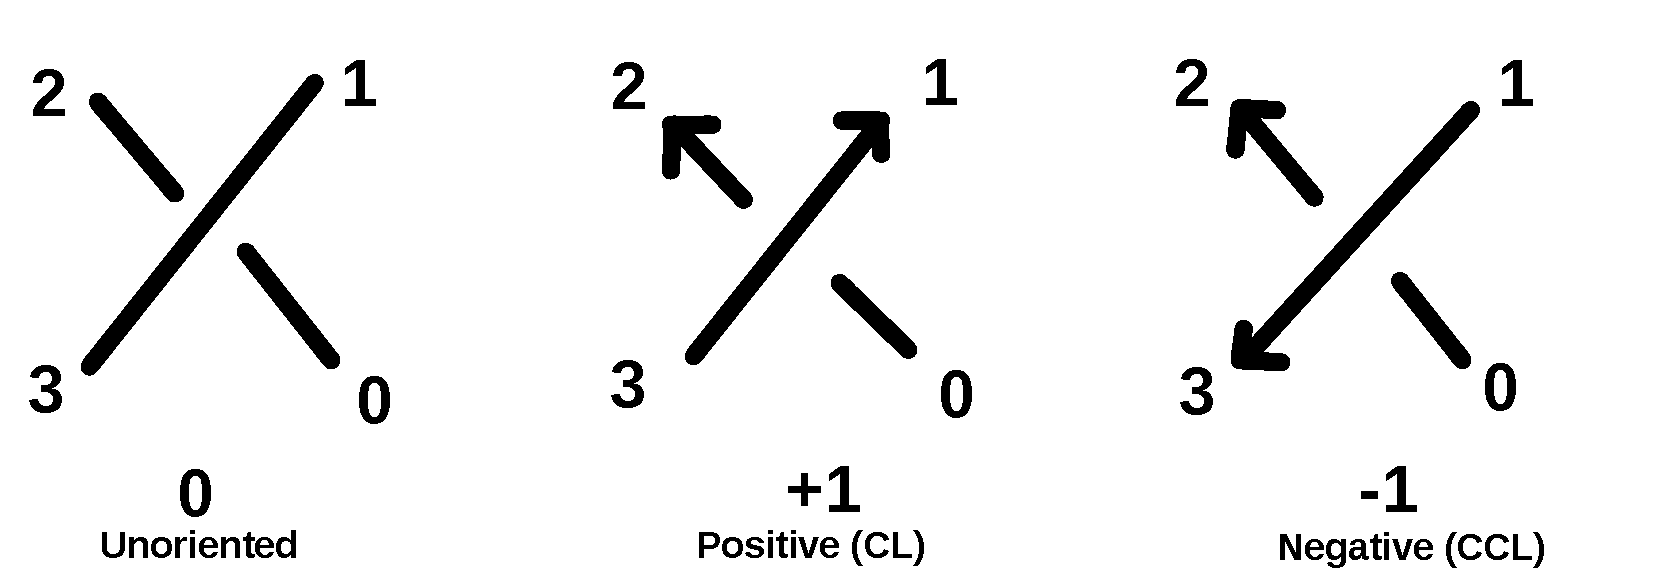
\includegraphics[scale=0.6]{pics/crossings}

\pagebreak

\section{Conventions for tangles}

Follows \url{http://homepages.math.uic.edu/~kauffman/VegasAMS.pdf
}

\begin{cxyoverpic}{(432,576)}{scale=1.0}{pics/tangles}
    ,(74,439)*{T + S}
    ,(183,418)*{T \ast S}
    ,(273,484)*{\mbox{\scriptsize cross.}}
    ,(273,500)*{\mbox{\scriptsize mirror}}
    ,(270,445)*{-T}
    ,(354,440)*{\displaystyle\frac{1}{T}}
    ,(126,282)*{\mbox{\normalsize Numerator closure}}
    ,(287,282)*{\mbox{\normalsize Denominator closure}}
    ,(20,235)*+!L{\mbox{\textbf{Basic rational tangles}}}
    ,(71,164)*{-2}
    ,(145,164)*{-1}
    ,(209,164)*{0}
    ,(282,164)*{1}
    ,(363,164)*{2}
    ,(69,76)*{\displaystyle -\frac{1}{2}}
    ,(152,76)*{\displaystyle-\frac{1}{1}}
    ,(212,74)*{\infty}
    ,(280,77)*{\displaystyle\frac{1}{1}}
    ,(364,74)*{\displaystyle\frac{1}{2}}
\end{cxyoverpic}


\end{document}

